\documentclass{sig-alternate}

\usepackage[utf8]{inputenc}
\usepackage[activate=compatibility]{microtype}

% autoref command
\usepackage[hyphens]{url}
\usepackage[pdftex,urlcolor=black,colorlinks=true,linkcolor=black,citecolor=black]{hyperref}
\def\sectionautorefname{Section}
\def\subsectionautorefname{Subsection}
\def\subfigureautorefname{Subfigure}

% Graphics
\usepackage{graphicx}
\usepackage{subfig}
\usepackage[font=small]{caption}
\captionsetup[figure]{name=Figure}
\usepackage{subcaption}

\usepackage{amsmath}
\usepackage{enumitem}
\usepackage{pbox}
\usepackage{color}
\definecolor{light-gray}{gray}{0.8}

% todo macro
\usepackage{color}
\newcommand{\todo}[1]{\noindent\textcolor{red}{{\bf \{TODO}: #1{\bf \}}}}

% nicer looking Google+
\usepackage{xspace}
\DeclareRobustCommand{\googleplus}{\mbox{Google\hspace{0em}\raisebox{.28ex}{\tiny\bf +}\kern-0.2ex}\xspace}

\DeclareRobustCommand{\plusone}{\mbox{\hspace{0em}\raisebox{.28ex}{\tiny\bf +}\kern-0.2ex 1}\xspace}

% listings and Verbatim environment
\usepackage{fancyvrb}
\usepackage{relsize}
\usepackage{listings}
\usepackage{verbatim}
\newcommand{\defaultlistingsize}{\fontsize{8pt}{9.5pt}}
\newcommand{\inlinelistingsize}{\fontsize{8pt}{11pt}}
\newcommand{\smalllistingsize}{\fontsize{7.5pt}{9.5pt}}
\newcommand{\listingsize}{\defaultlistingsize}
\RecustomVerbatimCommand{\Verb}{Verb}{fontsize=\inlinelistingsize}
\RecustomVerbatimEnvironment{Verbatim}{Verbatim}{fontsize=\defaultlistingsize}
\lstset{frame=lines,captionpos=b,numberbychapter=false,escapechar=§,
        aboveskip=2em,belowskip=1em,abovecaptionskip=0.5em,belowcaptionskip=0.5em,
        framexbottommargin=-1em,basicstyle=\ttfamily\listingsize\selectfont}

% use Courier from this point onward
\let\oldttdefault\ttdefault
\renewcommand{\ttdefault}{pcr}
\let\oldurl\url
\renewcommand{\url}[1]{\inlinelistingsize\oldurl{#1}}

\lstdefinelanguage{JavaScript}{
  keywords={push, typeof, new, true, false, catch, function, return, null, catch, switch, var, if, in, while, do, else, case, break},
  keywordstyle=\bfseries,
  ndkeywords={class, export, boolean, throw, implements, import, this},
  ndkeywordstyle=\color{darkgray}\bfseries,
  identifierstyle=\color{black},
  sensitive=false,
  comment=[l]{//},
  morecomment=[s]{/*}{*/},
  commentstyle=\color{darkgray},
  stringstyle=\color{red},
  morestring=[b]',
  morestring=[b]"
}

% linewrap symbol
\definecolor{grey}{RGB}{130,130,130}
\newcommand{\linewrap}{\raisebox{-.6ex}{\textcolor{grey}{$\hookleftarrow$}}}

\hyphenation{Wikistream Wikipedia Wikipedias}

%\def\baselinestretch{0.99}

\begin{document}

% --- Author Metadata here ---
\conferenceinfo{World Wide Web Conference}{'13 Rio de Janeiro, Brazil}
\CopyrightYear{2013} % Allows default copyright year (20XX) to be over-ridden - IF NEED BE.
%\crdata{0-12345-67-8/90/01}  % Allows default copyright data (0-89791-88-6/97/05) to be over-ridden - IF NEED BE.
% --- End of Author Metadata ---


\title{To Crop, Or Not to Crop: Creating Online Media Galleries}

\numberofauthors{2}\author{
\alignauthor
Thomas Steiner\\
	\affaddr{Google Germany GmbH}\\
	\affaddr{ABC-Str. 19}\\
	\affaddr{20354 Hamburg, Germany}\\
	\email{tomac@google.com} 
\alignauthor
Christopher Chedeau\\
	\affaddr{Facebook, Inc.}\\
	\affaddr{1601 Willow Road}\\
	\affaddr{Menlo Park, CA, 94025, USA}\\
	\email{vjeux@facebook.com} 
}
\maketitle

\begin{abstract}
We have developed an application for the automatic generation of
media galleries that visually and audibly summarize events
based on media items like videos and photos from multiple social networks.
We have evaluated different media gallery styles with online surveys 
and examined their pros and cons.
Besides the survey results, our contribution is also the application itself,
where media galleries of different styles can be created on-the-fly.
A~demo is available at
\url{http://social-media-illustrator.herokuapp.com/}.
\end{abstract}

\vspace{-1mm}
\category{H.3.3}{Information Search and Retrieval}{Clustering}

\vspace{-2mm}
\terms{Algorithms}

\vspace{-2mm}
\keywords{Media Galleries, Event Summarization, Social Networks}

\section{Introduction}
\label{sec:introduction}

Media galleries (see \autoref{fig:media-gallery} for two examples)
help people consume larger, however not overwhelmingly huge,
amounts of media items in an ideally pleasing and aesthetic way.
These media items may, or, more commonly, may not be ordered,
besides an intrinsic chronologic order.
In the context of our work on summarizing events
based on microposts and media items stemming from
multiple social networks, we have created means
to first \emph{extract} event-related media items
from multiple social networks, second, to
\emph{deduplicate} near- and exact-duplicate media items,
third, to \emph{cluster} them by visual similarity, and
finally, to \emph{rank} the resulting media item clusters
according to well-defined ranking criteria.
In this paper, we treat the challenge of \emph{compiling}
ranked media item clusters in media galleries in ways
such that the ranking-implied order is respected.
Previously, we have defined~\cite{steiner2012definingaesthetic}
aesthetic principles for automatic media gallery layout,
which we now apply to different media gallery types.

\section{Media Gallery Styles}

Media galleries---in contrast to free-form digital media collages---%
necessarily display media items in a~grid-like way.
The crucial question is thus, whether the media items' aspect ratios
should be respected, or whether they should be cropped to square,
or other aspect ratios (\emph{e.g.}, 4:3 or 16:9).
Respecting the aspect ratio has the advantage that media items
do not need to be potentially lossily cropped,
however, due to the unpredictable media item formats,
layouting of media galleries
that do not look frayed is harder.
The advantage of cropping is that media gallery layout is easier,
as the media item formats are predictably the same,
at the cost of having to decide where to crop.
Different algorithms (\emph{e.g.},~\cite{suh2003thumbnail})
beyond this paper's scope exist to aid this decision.
A~media gallery is \emph{balanced}, if its shape is rectangular,
\emph{hole-free} if there are no gaps from missing media items,
and \emph{order-respecting},
if media items appear in insertion order.

\subsection{Non-Order-Respecting Styles}

An interesting technique for arranging media items is dividing.
Every media item with an aspect ratio of $ \sqrt2 $ can be divided
into two media items with the same aspect ratio.%
\footnote{\url{http://blog.vjeux.com/2012/image/image-layout-algorithm-lightbox-android.html},
accessed 02/22/2013}
This works for portrait and landscape orientations,
however, is not order-respecting.
Two other non-order-respecting techniques are working
with pre-defined placeholder patterns
(small and big squares, portrait and landscape rectangles)
and then filling the placeholder shapes with media items,%
\footnote{\url{http://blog.vjeux.com/2012/image/image-layout-algorithm-500px.html},
accessed 02/22/2013}
or working with columns of pre-defined widths
and then iteratively inserting in the smallest column.%
\footnote{\url{http://blog.vjeux.com/2012/image/image-layout-algorithm-lightbox.html},
accessed 02/22/2013}
As outlined in \autoref{sec:introduction},
we need (loosely) order-respecting media galleries.

\subsection{Strict Order, Equal Size}

A~media gallery style that we call \emph{Strict Order, Equal Size},
which strictly respects the ranking-implied order is presented in~%
\cite{chedeau2012googleplus}.
An example can be seen in \autoref{fig:a}.
The algorithm works by resizing all media items in a~row to have the same height
and adjusting the widths so that the aspect ratios are maintained.
A~row is filled until a~maximum row height is reached,
then a~new row (with a~typically different height) starts, \emph{etc.}
This media gallery style is order-respecting, hole-free,
and can be easily balanced by adjusting the number
of media items in the gallery accordingly.

\begin{figure*}[t!]
  \centering
  \subfloat[Strict order, equal size]{
    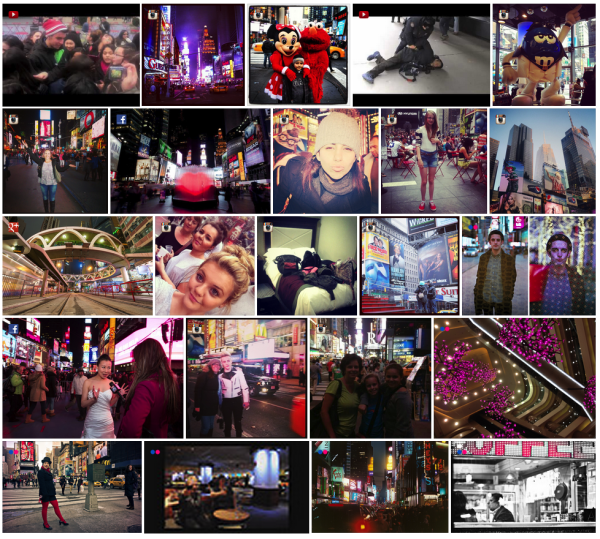
\includegraphics[height=4.5cm]{equal-size.png}
    \label{fig:a}
  }                
  \subfloat[Loose order, varying size (cropped)]{
    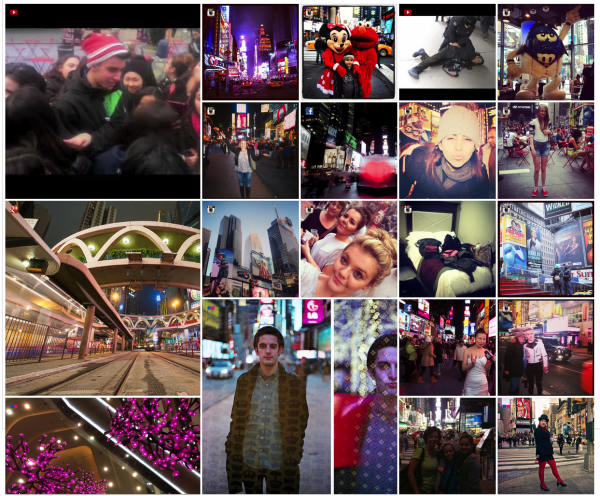
\includegraphics[height=4.5cm]{different-size.png}
    \label{fig:b}
  }
  \caption{Two different kinds of media galleries visualizing a~gathering at Times Square, New York on February 8, 2013}
  \label{fig:media-gallery}  
\end{figure*}

\subsection{Loose Order, Varying Size}

An example of a~media gallery style
that we call \emph{Loose Order, Varying Size}
can be seen in \autoref{fig:b},
with the details explained in~\cite{chedeau2012facebook}.
The algorithm works by cropping all images to a~square aspect ratio,
which allows organizing media items such that one big square
contains two horizontal lines of two small squares each.
The media gallery is formed by iteratively filling
big or small squares until a~square is full,
and then adding it to the smallest column.
This media gallery style allows any media item to become big,
while still being loosely order-respecting and always hole-free.
Balancing the gallery is harder,
as up to $ (\mathit{bigBlocksPerRow} - 1) \times 2 $ media items
may be required in the worst case.

\section{Discussion}

\section{Evaluation}

Evaluating subjective data, like \emph{the} correct presentation form
for a~set of media items, is a~challenging task.
For different users, there may be different optimal settings.
A~common subjective evaluation technique
is the Mean~Opinion Score (MOS,~\cite{itu1998mos}).
Traditionally, MOS is used for conducting subjective evaluations
of telephony network transmission quality,
however, recently MOS has also found
wider usage in the multimedia community
for evaluating \emph{per se} subjective things
like perceived quality from a~user perspective. 
Therefore, a~set of standard subjective tests are conducted,
where a~number of users rate the quality of test samples
with scores ranging from 1 (worst) to 5 (best).
The actual MOS is then the arithmetic mean of all individual scores.

\section{Conclusions and Future Work}

\bibliographystyle{abbrv}
\bibliography{www2013poster}

\end{document}